\subsection{ARM [Mohammed Mehedi Hasan]}

In Azure solutions, ARM(Azure Resource Manager) templates can be used for infrastructure as code. This service is developed and maintained by microsoft. The template is written in JSON format. This json file is responsible for defining infrastructure and configuration of the project. The project resources are defined in this ARM template. Therefore those resources are deployed with defined properties in the Resource Group. This mechanism reduce the overhead of creating those resources in recourse manager every time a deployment is needed. Furthermore, if any changes are required in the resources one just have to change the arm files and pushed the changes into branch since these files are kept into code repo.\footnote{https://docs.microsoft.com/en-us/azure/azure-resource-manager/templates/overview}

\subsubsection{ARM Template File}

In ARM Template file, one will use any or all of these five \textit{Parameters}, \textit{Variables}, \textit{User-defined functions}, \textit{Resources} and \textit{Outputs} definitions.\footnote{https://docs.microsoft.com/en-us/azure/azure-resource-manager/templates/overview}

Parameters are used to help construct the resources. "Resource Manager resolves parameter values before starting the deployment operations. Wherever the parameter is used in the template, Resource Manager replaces it with the resolved value."\footnote{https://docs.microsoft.com/en-us/azure/azure-resource-manager/templates/parameters}

One can use customised function to define a set of properties. By extend it can be used by multiple resources without defining those properties repeatedly. The name of this function has to be different from template built-in functions. \footnote{https://docs.microsoft.com/en-us/azure/azure-resource-manager/templates/user-defined-functions}

To create a resource one has to define the resource properties in the file. Resource type, api version, name, location, identity and many other properties can declare in resources.\footnote{https://docs.microsoft.com/en-us/azure/azure-resource-manager/templates/resource-declaration}

Variables are declared as values to use in the template files and it can also create by using parameters value.\footnote{https://docs.microsoft.com/en-us/azure/azure-resource-manager/templates/overview}

If any values are required from deployed resources then outputs need to be declared in the file.\footnote{https://docs.microsoft.com/en-us/azure/azure-resource-manager/templates/overview}

\subsubsection{Template Design}

One can design the templates as per the project requirement and design choice.
\begin{figure}[h]
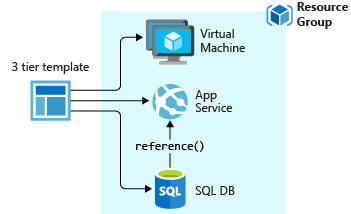
\includegraphics[scale=0.40]{images/mehedi/3-tier-template.png}
\centering
\caption{3 tier template}
\label{fig:3_tier_template}
\end{figure}

\begin{figure}[h]
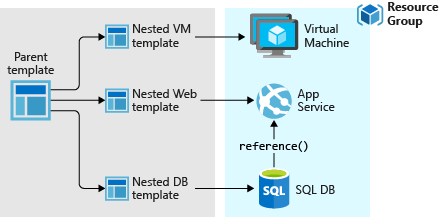
\includegraphics[scale=0.40]{images/mehedi/nested-tiers-template.png}
\centering
\caption{Nested tier template}
\label{fig:nested_tier_template}
\end{figure}

\begin{figure}[h]
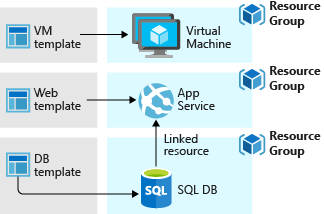
\includegraphics[scale=0.40]{images/mehedi/tier-templates.png}
\centering
\caption{tier template}
\label{fig:tier_template}
\end{figure}

As per figure \ref{fig:3_tier_template} one single template file can contain all the different resources in one resource group for deployment. In figure \ref{fig:nested_tier_template} same infrastructure can be designed in separate template files instead of a single one as well. Lastly according to figure \ref{fig:tier_template} the resources can deploy in separate resource groups and they can be linked with one another also.\footnote{https://docs.microsoft.com/en-us/azure/azure-resource-manager/templates/overview}

Using ARM template in azure CI/CD made the infrastructure update more reliable, faster and hassle free.